\documentclass[12pt,letterpaper]{article}

% ==============================================================================
% FORMATO APA 7MA EDICIÓN - UNIVERSIDAD TECNOLÓGICA DE PEREIRA
% ==============================================================================
\usepackage[utf8]{inputenc}
\usepackage[spanish,es-nodecimaldot,es-tabla]{babel}
\usepackage[top=2.00cm, bottom=1.80cm, left=2.20cm, right=2.20cm]{geometry}
\usepackage{graphicx}
\usepackage{booktabs}
\usepackage{tabularx}
\usepackage{fancyhdr}
\usepackage{float}
\usepackage{titlesec}
\usepackage{setspace}
\usepackage{enumitem}
\usepackage{amsmath}
\usepackage{hyperref}
\usepackage{mathptmx} % Times New Roman APA
\usepackage{caption}

% Formato de leyendas APA 7ma edición
\captionsetup{
    labelfont=bf,
    textfont=it,
    labelsep=newline,
    singlelinecheck=false,
    justification=raggedright,
    font=small,
    skip=4pt
}

\setlength{\headheight}{15pt}
\addtolength{\topmargin}{-3pt}
\setstretch{1.06} % Interlineado compacto y elegante APA

% Jerarquía de títulos limpia APA 7
\titleformat{\section}
  {\normalfont\Large\bfseries\centering}
  {}{0em}{}

\titleformat{\subsection}
  {\normalfont\large\bfseries}
  {}{0em}{}

\titleformat{\subsubsection}
  {\normalfont\normalsize\bfseries\itshape}
  {}{0em}{}

\titlespacing*{\section}{0pt}{0.8ex plus .2ex minus .2ex}{0.3ex}
\titlespacing*{\subsection}{0pt}{0.6ex plus .2ex minus .2ex}{0.25ex}
\titlespacing*{\subsubsection}{0pt}{0.5ex plus .1ex minus .1ex}{0.15ex}

% Encabezado formal APA
\pagestyle{fancy}
\fancyhf{}
\renewcommand{\headrulewidth}{0pt}
\fancyhead[R]{\small\thepage}
\fancyhead[L]{\small\textit{Capítulo II: Estudio de Mercado e Investigación -- Solar as a Service}}

\hypersetup{
    colorlinks=true,
    linkcolor=black,
    citecolor=black,
    urlcolor=blue
}

\begin{document}

% ==============================================================================
% PORTADA
% ==============================================================================
\begin{titlepage}
    \centering
    \vspace*{0.5cm}
    
    \begin{figure}[H]
        \centering
        
\includegraphics[width=0.45\textwidth]{../assets/UTP_color.png}
    \end{figure}
    
    \vspace{0.8cm}
    
    {\Large\bfseries Estudio de Mercado e Investigación de Mercados:}\\[0.2cm]
    {\Large\bfseries Modelo Solar as a Service (SaaS) en Pereira}\\[0.4cm]
    {\large Avance Académico -- Capítulo II (Secciones 2.1 y 2.2)}\\[1.8cm]
    
    {\normalsize\bfseries Integrantes:}\\[0.2cm]
    {\normalsize Juan Esteban Nieto Valencia}\\
    {\normalsize José Daniel Ruíz Gómez}\\
    {\normalsize Jose David Toro Naranjo}\\[1.8cm]
    
    {\normalsize Facultad de Ingenierías, Programa de Ingeniería Eléctrica}\\
    {\normalsize Asignatura: Formulación y Evaluación de Proyectos}\\
    {\normalsize Universidad Tecnológica de Pereira}\\[1.0cm]
    
    {\normalsize Octubre de 2026}
\end{titlepage}

\newpage
\pagenumbering{arabic}

% ==============================================================================
% CONTENIDO PRINCIPAL: PARTE 2.1
% ==============================================================================
\section{Capítulo II: Estudio de Mercado}

\subsection{2.1 Estudio de Mercado: Caracterización y Modelo Comercial}

Este capítulo presenta el estudio de mercado para la creación de una empresa de energía solar bajo el modelo de suscripción mensual (\textbf{Solar as a Service}) en Pereira. 

La idea central del proyecto es eliminar la barrera económica que impide a pequeños negocios y fincas instalar paneles solares. En lugar de exigirles una compra de contado de \$40 o \$100 millones de pesos, la empresa instala el sistema completo sin costo inicial (\$0 cuota de entrada), se encarga del mantenimiento y seguros, y cobra una \textbf{cuota fija mensual predecible} que garantiza un ahorro inmediato frente a lo que pagan hoy en su factura eléctrica.

\vspace{0.2cm}

\subsubsection{2.1.1 Diagnóstico del Mercado}

En Pereira existen tres condiciones clave que hacen viable este modelo:
\begin{enumerate}[leftmargin=1.5em, itemsep=2pt]
    \item \textbf{Tarifas de energía elevadas:} La Empresa de Energía de Pereira (EEP) cobra en promedio \textbf{\$980 COP por kWh} al sector comercial e industrial (incluyendo la contribución legal del 20\%). Para negocios con refrigeración o producción diurna, la luz representa uno de sus mayores costos fijos.
    \item \textbf{Excelente recurso solar:} La ciudad recibe un promedio diario de radiación solar de \textbf{4,88 kWh/m$^2$}, con una alta estabilidad climática a lo largo del año que permite generar energía limpia en el mismo techo donde se consume (véase Figura~\ref{fig:recurso_solar}).
    \item \textbf{Leyes favorables:} La legislación colombiana (Ley 1715 de 2014, Ley 2099 de 2021 y normas CREG) permite conectar los paneles a la red para intercambiar energía sin necesidad de costosas baterías químicas, y exime a los equipos de aranceles e IVA.
\end{enumerate}

De acuerdo con la Cámara de Comercio de Pereira (2025), en la jurisdicción regional de Risaralda existen más de \textbf{50.000 unidades productivas} registradas (\textit{Total Addressable Market}, TAM). Delimitando este universo al municipio de Pereira, se identifican cerca de \textbf{25.000 establecimientos comerciales y de servicios formalmente activos} (\textit{universo censal base $N$}). De estos, un subconjunto de aproximadamente \textbf{3.200 pequeños comercios y fincas} presentan cubiertas técnicamente aptas y consumos diurnos intensivos (\textit{Serviceable Addressable Market}, SAM). La meta comercial inmediata del proyecto es consolidar un portafolio piloto inicial de \textbf{20 clientes comerciales y rurales} (\textit{Serviceable Obtainable Market}, SOM).

\begin{figure}[H]
    \caption{Potencial y estabilidad de la radiación solar mensual en Pereira}\label{fig:recurso_solar}
    \centering
    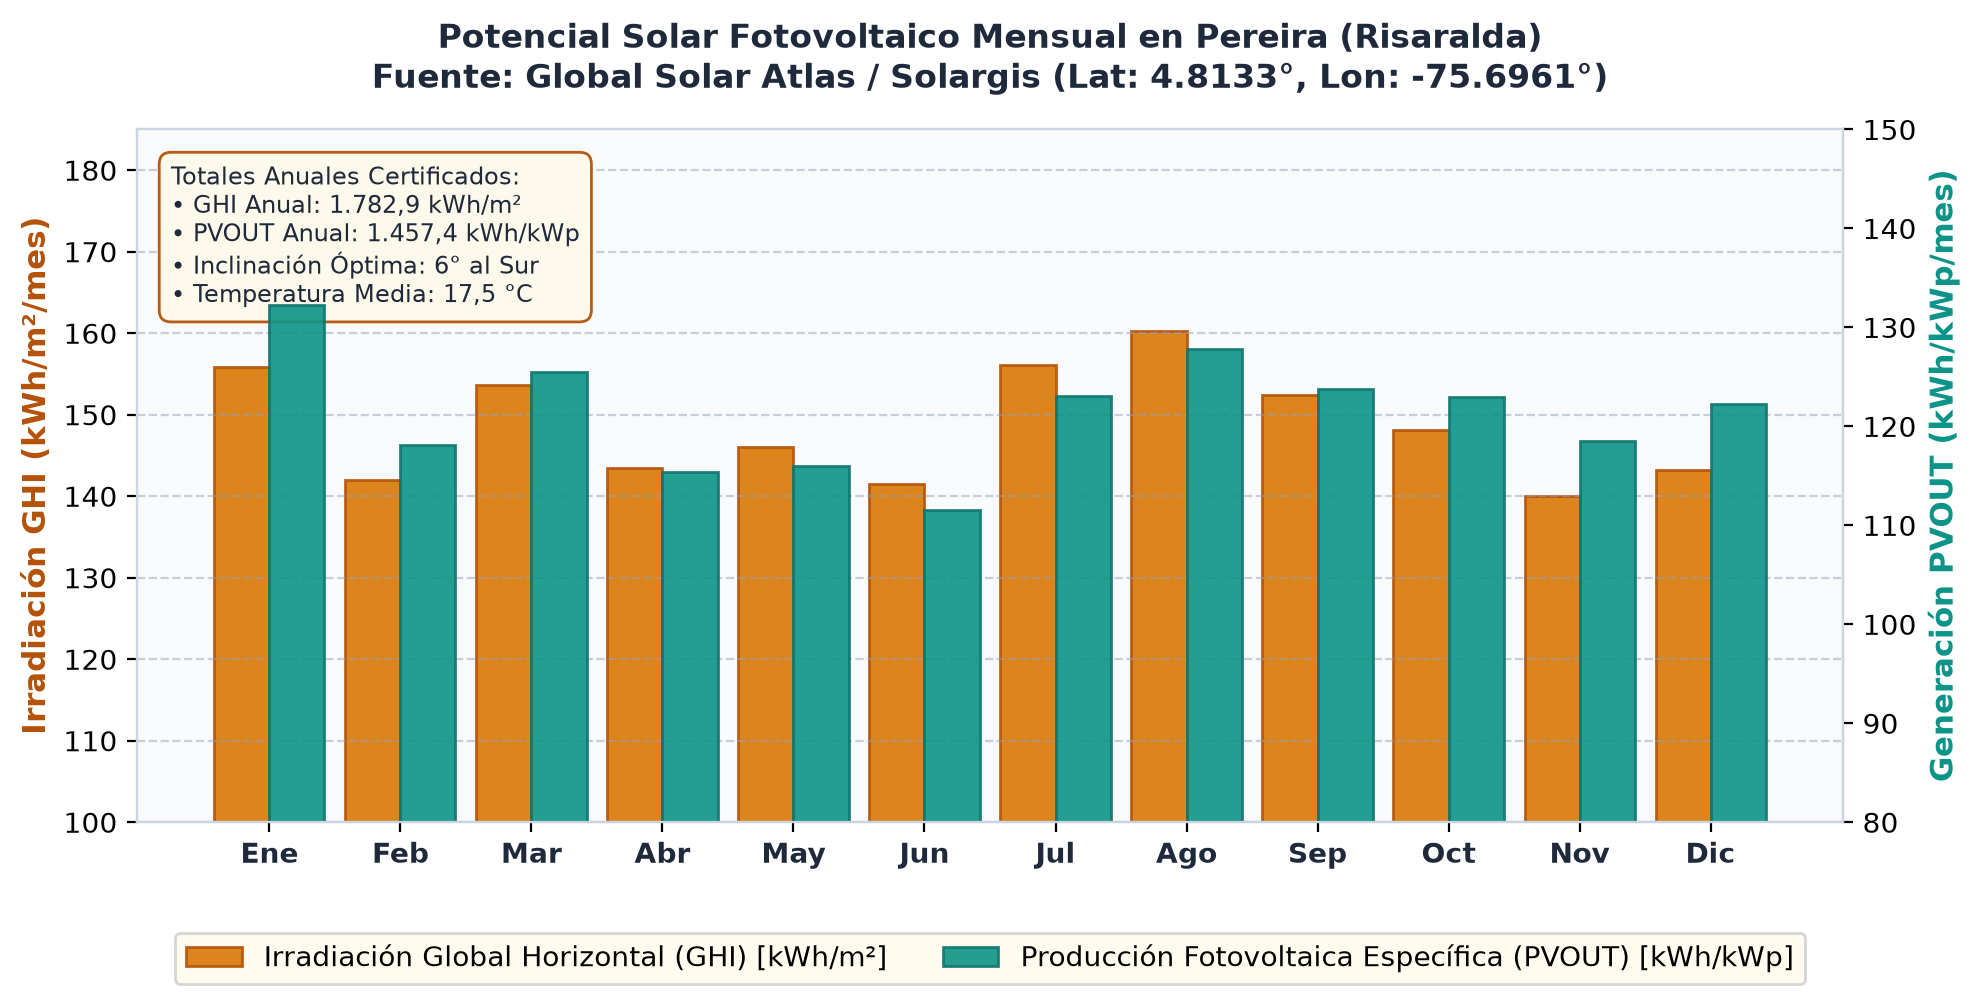
\includegraphics[width=0.72\textwidth]{../assets/mapa_recurso_solar_pereira.png}
    \vspace{0.15cm}
    \raggedright
    \footnotesize\textit{Nota.} Radiación solar global horizontal (GHI) y rendimiento fotovoltaico específico (PVOUT) multianual satelital para Pereira. Adaptado de Global Solar Atlas y Solargis (2026).
\end{figure}

\subsubsection{2.1.2 Clientes Objetivo y Bancabilidad}

El servicio se enfoca en tres tipos de clientes comerciales y rurales con alta demanda eléctrica diurna, cuyas características operativas y necesidades críticas se detallan en la Tabla~\ref{tab:segmentos}:

\begin{table}[H]
\small
\renewcommand{\arraystretch}{1.15}
\caption{Segmentos de clientes comerciales y rurales priorizados en Pereira}\label{tab:segmentos}
\vspace{0.15cm}
\centering
\begin{tabularx}{\textwidth}{p{3.2cm} p{3.5cm} X}
\toprule
\textbf{Segmento} & \textbf{Negocios Típicos} & \textbf{Necesidad Principal} \\
\midrule
\textbf{Comercio con Frío} & Panaderías, minimercados y carnicerías & Reducir la factura de luz mensual sin descapitalizarse ni sacar préstamos. \\
\textbf{Fincas y Agroindustria} & Fincas cafeteras, avícolas y hoteles rurales & Aprovechar cubiertas grandes y contar con soporte técnico confiable en el campo. \\
\textbf{Pequeña Industria} & Talleres de metalmecánica y confección & Bajar costos en sus horarios de mayor trabajo diurno. \\
\bottomrule
\end{tabularx}
\vspace{0.15cm}
\raggedright
\footnotesize\textit{Nota.} Elaboración propia a partir de datos del Censo Empresarial (Cámara de Comercio de Pereira, 2025).
\end{table}

Para garantizar la bancabilidad ante las líneas de crédito verde (Findeter) y mitigar el riesgo de impago, los clientes deben ser \textbf{propietarios del inmueble} o contar con un \textbf{codeudor solvente con finca raíz}, respaldando el contrato mediante pagaré y registro prendario en el \textbf{RUG (Ley 1676 de 2013)} ante Confecámaras.

\subsubsection{2.1.3 Análisis de la Competencia}

Actualmente, las empresas solares en el Eje Cafetero operan bajo dos esquemas tradicionales:
\begin{itemize}[leftmargin=1.5em, itemsep=2pt]
    \item \textbf{Venta de contado o crédito (EPC):} Exigen desembolsar entre \$30 y \$120 millones de pesos por adelantado, dejando por fuera a la mayoría de pymes que no tienen esa liquidez.
    \item \textbf{Grandes contratos de energía (PPA):} Solo atienden a multinacionales e industrias muy grandes con contratos a 15 o 20 años.
\end{itemize}

El modelo \textbf{Solar as a Service} se diferencia ofreciendo: inversión inicial de \$0 COP, mantenimiento y seguros a cargo de la empresa, y traslado de paneles con permanencia mínima de 36 meses (cubriendo el usuario los costos de re-adecuación y RETIE).

\subsubsection{2.1.4 Fuentes de Información}

Para este estudio se consultaron fuentes oficiales: pliegos tarifarios de la Empresa de Energía de Pereira (EEP), bases estadísticas de la Cámara de Comercio de Pereira, radiación satelital del Banco Mundial / Global Solar Atlas y la Resolución CREG 174 de 2021.

\subsubsection{2.1.5 Estrategia de Mercado y Marketing Mix (4Ps)}

Se adopta una estrategia de enfoque, iniciando con pequeños comercios en zonas urbanas de Pereira y expandiéndose hacia fincas campestres en Cerritos y Combia:

\begin{enumerate}[leftmargin=1.5em, itemsep=2.5pt]
    \item \textbf{Producto (Tecnología 100\% On-Grid):} La empresa suministra un servicio integral de energía solar interconectado a la red (\textit{On-Grid}), sin baterías químicas que encarezcan el sistema en un 73\%. Se utiliza la red de EEP como \textbf{batería virtual} mediante la Resolución CREG 174 de 2021: el 80\% de la energía se autoconsume de día y el 20\% sobrante se inyecta a la red como Excedente Tipo 1 (compensación 1 a 1 en kWh), comportamiento horario de acoplamiento que se ilustra en la Figura~\ref{fig:curva_demanda}.
    
    \begin{figure}[H]
        \caption{Acoplamiento energético: Generación solar vs. demanda comercial típica en Pereira (15 kWp)}\label{fig:curva_demanda}
        \centering
        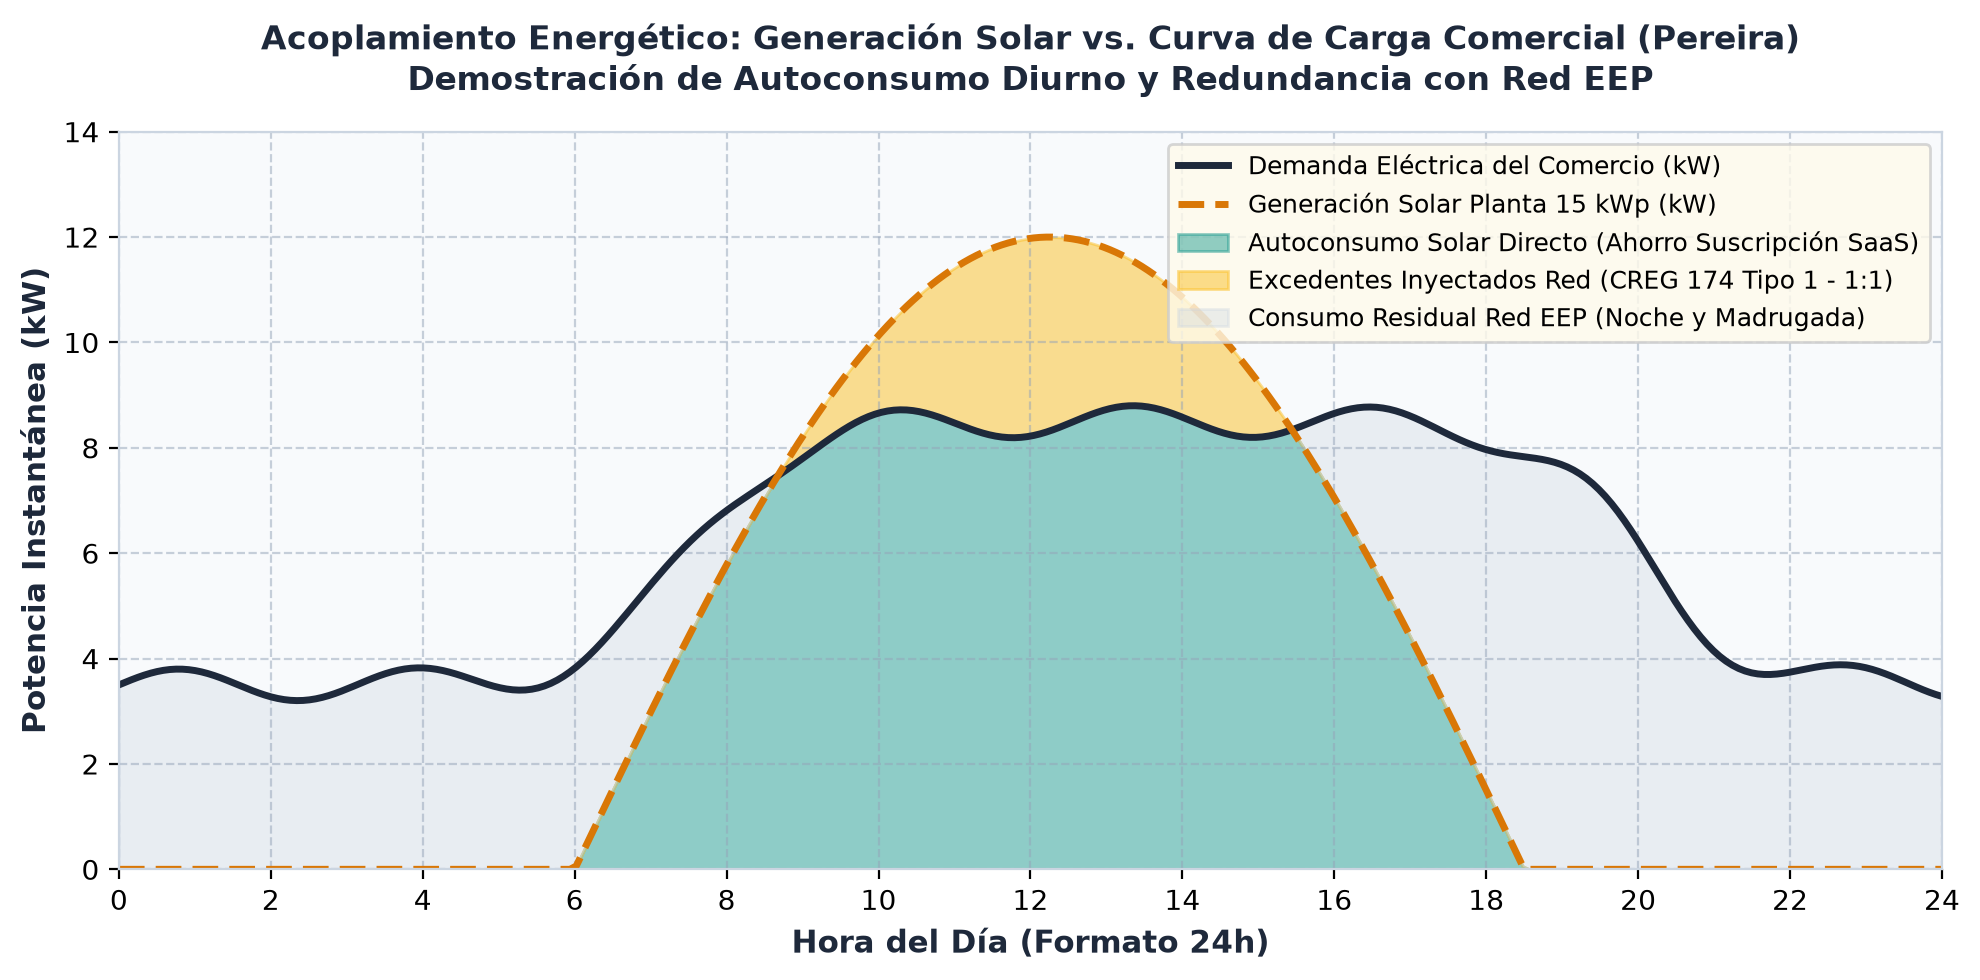
\includegraphics[width=0.70\textwidth]{../assets/curva_generacion_vs_demanda.png}
        \vspace{0.15cm}
        \raggedright
        \footnotesize\textit{Nota.} Simulación horaria de autoconsumo solar diurno e inyección de excedentes bajo la Resolución CREG 174 de 2021 para un perfil comercial típico de 15 kWp.
    \end{figure}
    
    \textbf{Valor Agregado (Vida Útil y Transferencia de Propiedad):} Los paneles TOPCon tienen una vida útil superior a \textbf{25 a 30 años}. Al culminar el contrato de suscripción de \textbf{8 años (mes 96)}, tras amortizarse la deuda bancaria, \textbf{la propiedad total de los equipos se transfiere al cliente sin costo adicional}, dejándole más de 15 años de energía gratuita con opción de mantenimiento preventivo anual económico.
    
    \item \textbf{Precio (Suscripción Fija y Ahorro):} Se cobra una \textbf{cuota fija mensual de \$1.250.000 COP} (15 kWp). Al descontar 1.870 kWh/mes generados frente a un consumo de 2.200 kWh, la factura de EEP baja de \$2.156.000 a \$324.000 COP. Sumando aseo y alumbrado (\$130.000), el gasto consolidado pasa de \$2.286.000 a \$1.704.000 COP, logrando un \textbf{ahorro neto de bolsillo de \$582.000 COP/mes (25,5\% de ahorro real)}, cuya estructura comparativa de facturación dual se desglosa en la Figura~\ref{fig:desglose_ahorro}.
    
    \begin{figure}[H]
        \caption{Desglose comparativo de facturación mensual: Antes vs. Con Solar as a Service (Facturación dual CREG 174)}\label{fig:desglose_ahorro}
        \centering
        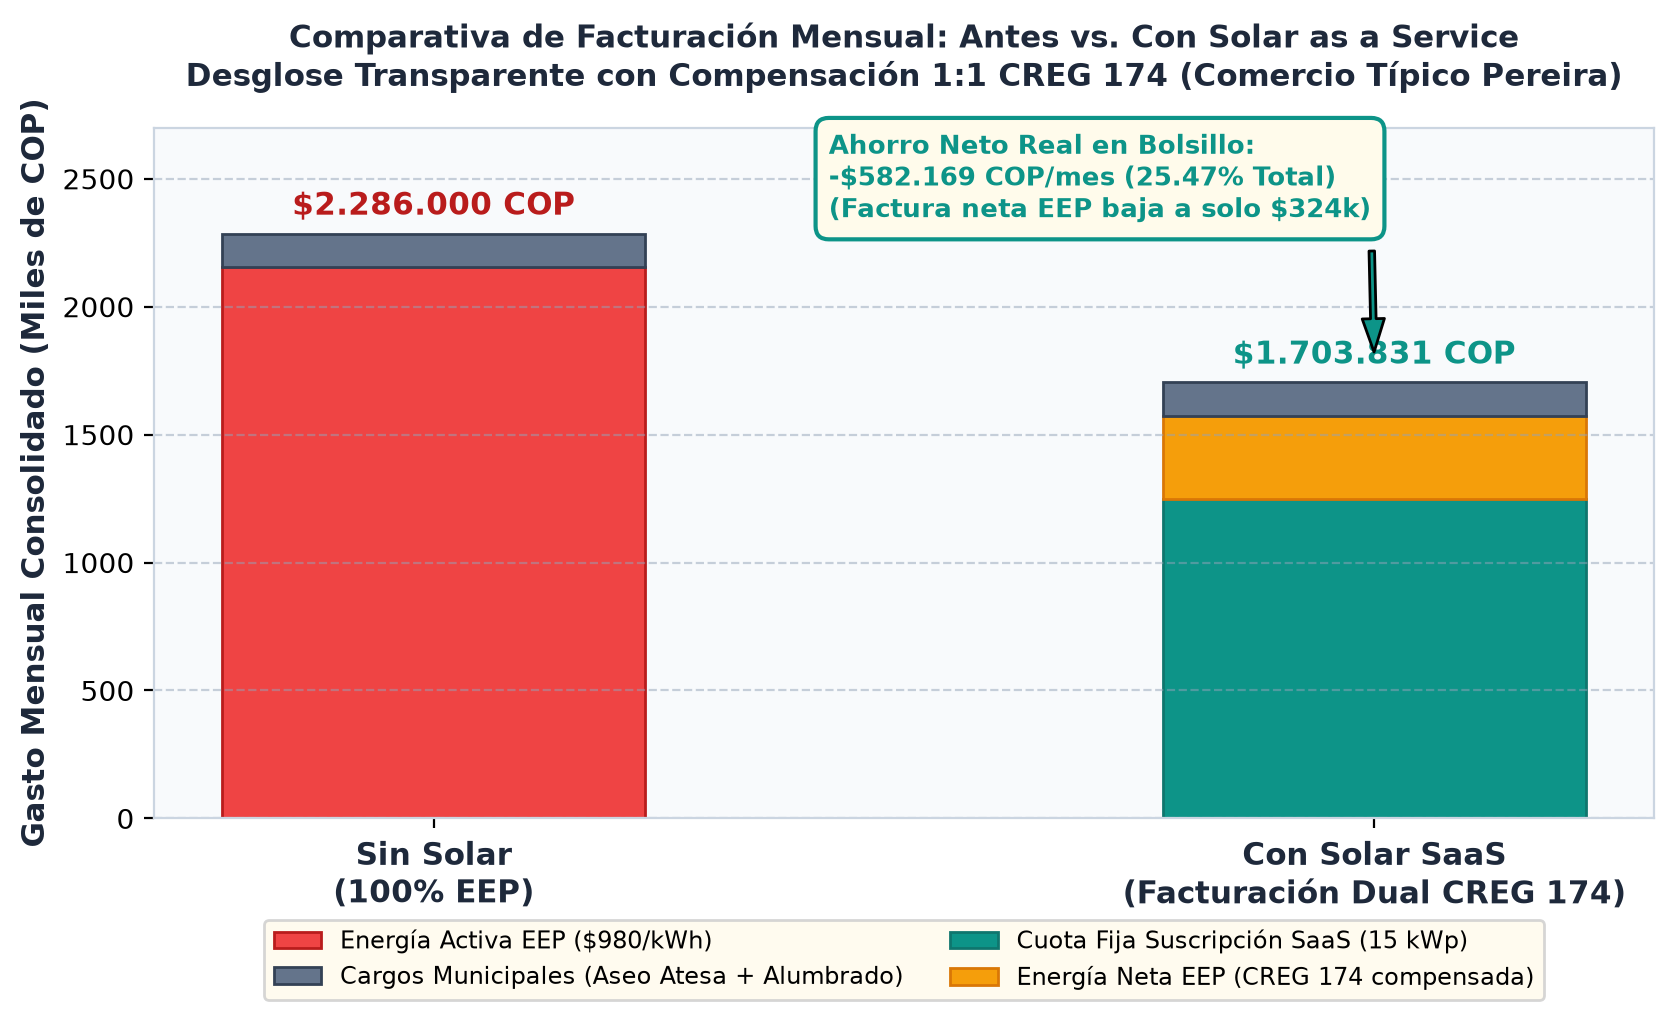
\includegraphics[width=0.64\textwidth]{../assets/desglose_ahorro_factura_dual.png}
        \vspace{0.15cm}
        \raggedright
        \footnotesize\textit{Nota.} Comparación mensual de gasto eléctrico para un usuario comercial de 2.200 kWh/mes con tarifa regulada EEP Nivel 1 (\$980 COP/kWh con contribución) vs. cuota fija SaaS y balance neto.
    \end{figure}
    
    \item \textbf{Distribución (Plaza):} Venta directa con ingenieros asesores que visitan al comerciante y analizan su recibo en mano, sumado a alianzas gremiales con Fenalco Risaralda y comités agrícolas.
    
    \item \textbf{Promoción:} Diagnóstico técnico gratuito in situ (\textit{Fast Assessment}) para inspeccionar la cubierta y certificar el ahorro real antes de la firma.
\end{enumerate}

\paragraph{Viabilidad Financiera del Portafolio Piloto (20 Clientes):}
Para respaldar la solidez del modelo ante las entidades bancarias (líneas de crédito verde Findeter al 70\% de deuda comercial), se modeló el flujo de fondos a 10 años para el portafolio piloto inicial de 20 clientes (300 kWp instalados). Como se evidencia en la Figura~\ref{fig:flujo_caja}, el portafolio demanda un capital propio inicial (\textit{equity}) de -\$306,81 millones COP, cubre holgadamente el servicio de deuda de \$157,9 millones COP anuales (con un indicador de cobertura DSCR de 1,53x en el Año 1, superando el estándar bancario de 1,25x), y logra su punto de equilibrio patrimonial (\textit{payback equity}) en el \textbf{Año 2,66 (~32 meses / 2 años y 8 meses)}. Con un costo de capital (WACC) del 13,5\%, el portafolio entrega un Valor Presente Neto (\textbf{VPN}) de \textbf{+\$380,27 millones COP} y una Tasa Interna de Retorno (\textbf{TIR Equity}) del \textbf{39,29\%}, demostrando que transferir el activo al usuario en el mes 96 es plenamente sostenible y rentable.

\begin{figure}[H]
    \caption{Proyección financiera a 10 años: Evolución de caja libre, amortización y transferencia de activo en año 8 (Portafolio 20 clientes)}\label{fig:flujo_caja}
    \centering
    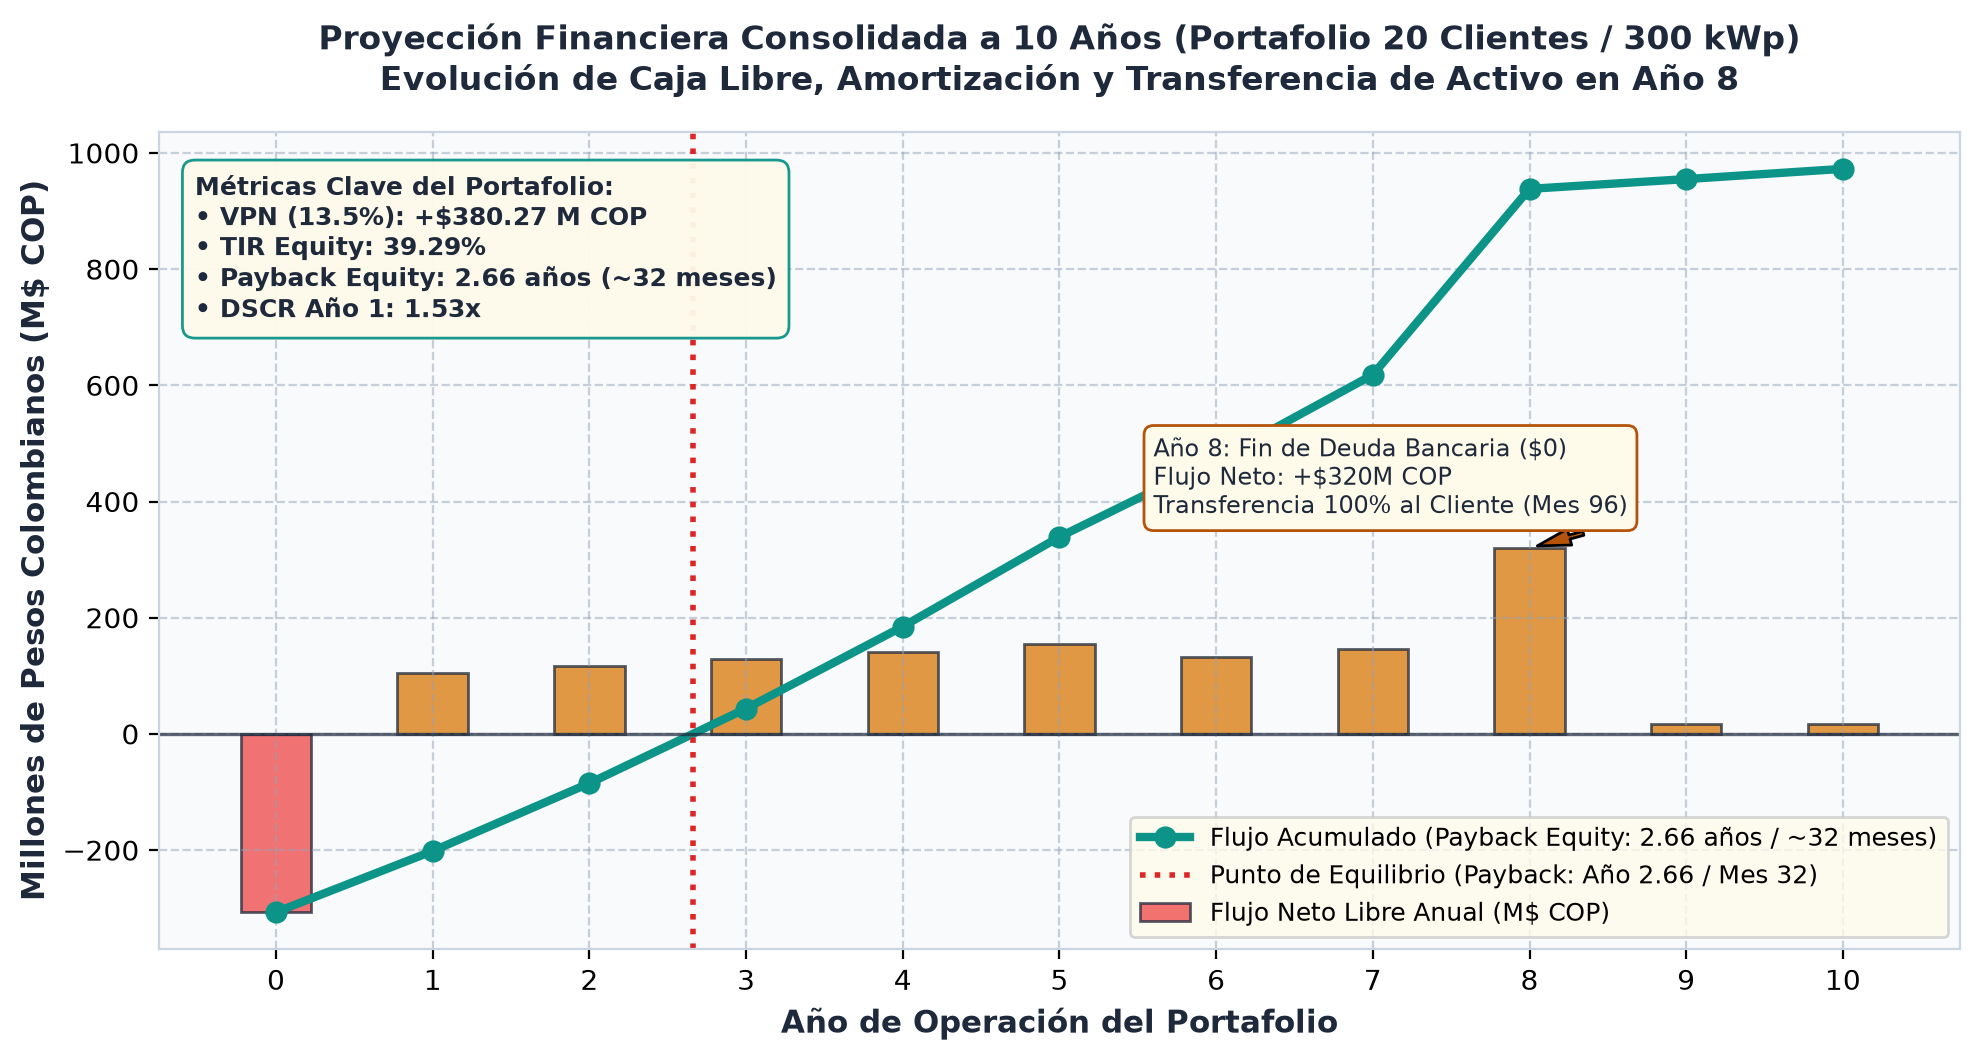
\includegraphics[width=0.70\textwidth]{../assets/flujo_caja_payback_10anios.png}
    \vspace{0.15cm}
    \raggedright
    \footnotesize\textit{Nota.} Proyección financiera del portafolio piloto (20 sistemas comerciales de 15,4 kWp). Muestra el flujo neto anual, el flujo acumulado con punto de equilibrio en el Año 2,66 (~32 meses), fin de deuda bancaria en el Año 7 (mes 84) y transferencia libre de la propiedad del activo al cliente en el Año 8 (mes 96).
\end{figure}

\subsubsection{2.1.6 Manejo de Variaciones de Consumo (Casos Extraordinarios)}

Para proteger la estabilidad del negocio, se establecen dos reglas contractuales transparentes:
\begin{itemize}[leftmargin=1.5em, itemsep=2pt]
    \item \textbf{Si el cliente aumenta su consumo:} El sistema solar sigue entregando su cuota y el excedente lo asume la red de EEP a tarifa normal. Si requiere más energía, puede solicitar una ampliación de paneles.
    \item \textbf{Si el cliente disminuye su consumo:} El sistema inyecta más energía a la red de EEP bajo CREG 174. El crédito liquidado por EEP se abona a la cuota del cliente en la siguiente factura, garantizando equidad.
\end{itemize}

\vspace{0.4cm}

% ==============================================================================
% SECCIÓN 2.2: INVESTIGACIÓN DE MERCADOS
% ==============================================================================
\subsection{2.2 Investigación de Mercados}

Una vez diagnosticada la oportunidad y estructurada la propuesta comercial preliminar en la sección precedente (2.1) con base en fuentes secundarias oficiales y predimensionamiento de ingeniería, la presente sección (2.2) formaliza el diseño metodológico de la investigación de mercados, fundamentando las técnicas de recolección y la representatividad estadística ($n = 379$) requerida para la verificación empírica en campo.

\subsubsection{2.2.1 Definición del Problema}

En Pereira, muchos pequeños negocios tienen gastos mensuales elevados en electricidad. Aunque los paneles solares pueden ayudar a reducir estos gastos, comprarlos e instalarlos requiere una inversión inicial que la mayoría de los comerciantes no pueden asumir. Además, quienes trabajan en locales arrendados enfrentan barreras legales y financieras para instalar activos fijos en inmuebles de terceros.

Por ello, \textbf{Solar Service} busca ofrecer paneles solares mediante un esquema de suscripción mensual que incluye diseño, instalación, monitoreo y mantenimiento continuo, eliminando la necesidad de que el cliente realice desembolsos de capital por adelantado.

\subsubsection{2.2.2 Planteamiento de Objetivos}

\textbf{Objetivo General:}
Analizar la viabilidad y oportunidad de mercado en Pereira para la provisión de sistemas solares fotovoltaicos mediante el modelo de pago por suscripción mensual (Solar as a Service).

\textbf{Objetivos Específicos:}
\begin{itemize}[leftmargin=1.5em, itemsep=2pt]
    \item Analizar la evolución y estructura de las tarifas comerciales de energía de la Empresa de Energía de Pereira (EEP).
    \item Identificar las tipologías de negocios y sectores productivos con mayor potencial de aprovechamiento diurno del servicio.
    \item Cuantificar la población objetivo y determinar el tamaño muestral representativo para estudios de campo.
    \item Evaluar los mecanismos contractuales y de garantías para la viabilidad de instalaciones en inmuebles comerciales y rurales.
    \item Determinar la estructura de ahorro neto del cliente frente al pago de la cuota mensual del servicio.
\end{itemize}

\subsubsection{2.2.3 Definición de la Población o Grupo de Estudio}

La población de estudio está conformada por micro, pequeños y medianos establecimientos comerciales, talleres y unidades agroproductivas de Pereira que presentan consumo eléctrico diurno significativo y cuentan con cubiertas técnicamente viables. Se priorizan panaderías, minimercados, carnicerías, talleres de manufactura y fincas rurales.

Como universo censal de referencia para el municipio de Pereira, se toma una población estimada de \textbf{25.000 establecimientos activos} (comercio formal y servicios), delimitada a partir de los cruces de microdatos de la Cámara de Comercio de Pereira (2025) y la Encuesta de Micronegocios (EMICRON) del DANE (2024).

\subsubsection{2.2.4 Definición y Cálculo del Tamaño de la Muestra}

Para calcular el tamaño muestral probabilístico representativo se utiliza la formulación estándar para poblaciones finitas (Levin \& Rubin, 2010):

\begin{equation}
n = \frac{N \cdot Z^2 \cdot p \cdot q}{e^2 \cdot (N - 1) + Z^2 \cdot p \cdot q}
\end{equation}

Donde los parámetros metodológicos corresponden a:
\begin{itemize}[leftmargin=1.5em, itemsep=1pt]
    \item $N = 25.000$ (universo total de establecimientos de comercio y servicios en Pereira).
    \item $Z = 1,96$ (nivel de confianza del 95\%).
    \item $p = 0,5$ (probabilidad estimada a favor de adopción del servicio).
    \item $q = 1 - p = 0,5$ (probabilidad en contra).
    \item $e = 0,05$ (margen de error máximo permitido del 5\%).
\end{itemize}

Reemplazando los valores cuantitativos y desarrollando los términos intermedios:

\begin{equation}
n = \frac{25.000 \cdot (1,96)^2 \cdot 0,5 \cdot 0,5}{(0,05)^2 \cdot (25.000 - 1) + (1,96)^2 \cdot 0,5 \cdot 0,5} = \frac{24.010}{62,4975 + 0,9604} = \frac{24.010}{63,4579} \approx 378,36
\end{equation}

En la teoría estadística de muestreo (Levin \& Rubin, 2010), el tamaño muestral resultante siempre debe \textbf{redondearse al entero superior inmediato} ($\lceil 378,36 \rceil = 379$). Este criterio garantiza formalmente que el margen de error real permanezca estrictamente acotado en $e \le 5,00\%$ (de haberse truncado a 378, el error real aumentaría a $5,0023\%$). Por lo tanto, la muestra formal representativa se fija en \textbf{379 establecimientos}, estableciendo el parámetro de rigor para encuestas primarias de validación en campo.

\subsubsection{2.2.5 Fuentes de Información}

La investigación se sustenta en fuentes secundarias oficiales y verificables del sector energético y económico:
\begin{itemize}[leftmargin=1.5em, itemsep=1.5pt]
    \item \textbf{Empresa de Energía de Pereira (EEP):} Pliegos tarifarios históricos y vigentes del mercado regulado no residencial y guías de conexión AGPE.
    \item \textbf{Cámara de Comercio de Pereira:} Registros del Censo Empresarial sobre densidad comercial, mortalidad empresarial y formalización en Risaralda.
    \item \textbf{Departamento Administrativo Nacional de Estadística (DANE):} Microdatos de la Encuesta de Micronegocios (EMICRON) sobre consumo de servicios públicos y tenencia de locales.
    \item \textbf{Comisión de Regulación de Energía y Gas (CREG):} Resolución CREG 174 de 2021 sobre autogeneración a pequeña escala e inyección de excedentes.
    \item \textbf{Global Solar Atlas (Banco Mundial / Solargis):} Base de datos satelital sobre irradiación horizontal (GHI) y potencial fotovoltaico (PVOUT) en Pereira.
\end{itemize}

\subsubsection{2.2.6 Instrumentos de Recolección}

El instrumento implementado es una \textbf{matriz de análisis documental y financiero}, diseñada para sistematizar y contrastar la información técnica y económica recopilada. A través de este instrumento se cruzan las tarifas de energía facturadas, la curva de carga diurna de los comerciantes, los costos de inversión llave en mano (CAPEX), los gastos operativos de seguros y mantenimiento (OPEX), y los ahorros netos proyectados para cada segmento de clientes.

\subsubsection{2.2.7 Análisis de la Información Recolectada}

El análisis confirma que la tarifa eléctrica comercial (\$980 COP/kWh con sobretasa legal) representa una de las mayores cargas operativas para los micro y pequeños empresarios en Pereira.

Los establecimientos comerciales con cadenas de frío (panaderías, carnicerías, minimercados) y talleres con maquinaria en operación continua coinciden exactamente con la curva de irradiación solar local (8:00 a.m. a 5:00 p.m.), maximizando el autoconsumo directo y la rentabilidad del servicio.

En cuanto a la tenencia de inmuebles, la presencia de locales arrendados exige que los contratos se suscriban con el propietario del predio o con un codeudor solvente con finca raíz, integrando garantías mobiliarias bajo la Ley 1676 de 2013 para blindar el financiamiento bancario del sistema.

\subsubsection{2.2.8 Hallazgos Principales}

\begin{enumerate}[leftmargin=1.5em, itemsep=1.5pt]
    \item \textbf{Alta sensibilidad a la factura energética:} Interés generalizado en el comercio de Pereira por reducir sus costos de electricidad debido a las continuas alzas tarifarias.
    \item \textbf{Barrera de liquidez inicial:} El modelo tradicional de paneles de contado (EPC) excluye a más del 90\% de los pequeños comerciantes por falta de capital de trabajo.
    \item \textbf{Viabilidad de la suscripción fija:} La cuota fija mensual integral (\$1.250.000 COP para 15 kWp) elimina la incertidumbre comercial y proporciona un ahorro neto superior al 25\% en bolsillo.
    \item \textbf{Aprovechamiento normativo sin baterías:} La Resolución CREG 174 de 2021 permite prescindir de costosas baterías de litio, utilizando la red de EEP como batería virtual de intercambio 1 a 1 sin costo.
    \item \textbf{Incentivo de transferencia patrimonial:} Transferir la propiedad de los paneles al cliente en el año 8 (mes 96), una vez amortizada la deuda bancaria, constituye el mayor argumento de cierre comercial frente a alternativas de alquiler indefinido.
\end{enumerate}

\vspace{0.25cm}
\hrule
\vspace{0.15cm}

\noindent\textbf{\small Nota de Trazabilidad y Metodología:}\\
{\footnotesize La memoria de cálculo financiero en Excel y la documentación de la investigación asistida por IA (con el registro de prompts y fuentes oficiales) se encuentran en el anexo de soporte metodológico.}

\vspace{0.25cm}

% ==============================================================================
% REFERENCIAS APA
% ==============================================================================
\section*{Referencias}

\begingroup
\small
\setlength{\parindent}{0pt}
\setlength{\hangindent}{1.27cm}
\newcommand{\refitem}[1]{\hangafter=1 #1\vspace{0.25em}\par}

\refitem{Cámara de Comercio de Pereira. (2025). \textit{Censo Empresarial e Informe de Dinámica Empresarial de Risaralda}. \url{https://camarapereira.org.co/es/censoempresarial}}

\refitem{Comisión de Regulación de Energía y Gas. (2021). \textit{Resolución CREG 174 de 2021: Por la cual se regulan las actividades de autogeneración a pequeña escala y de generación distribuida en el Sistema Interconectado Nacional}. CREG. \url{https://gestornormativo.creg.gov.co/gestor/entorno/docs/resolucion_creg_0174_2021.htm}}

\refitem{Congreso de la República de Colombia. (2013). \textit{Ley 1676 de 2013: Por la cual se promueve el acceso al crédito y se dictan normas sobre garantías mobiliarias}. Diario Oficial No. 48.888.}

\refitem{Congreso de la República de Colombia. (2014). \textit{Ley 1715 de 2014: Por medio de la cual se regula la integración de las energías renovables no convencionales al Sistema Energético Nacional}. Diario Oficial No. 49.150.}

\refitem{Departamento Administrativo Nacional de Estadística. (2024). \textit{Encuesta de Micronegocios (EMICRON) - Características de micronegocios y servicios públicos}. DANE. \url{https://microdatos.dane.gov.co/index.php/catalog/914}}

\refitem{Empresa de Energía de Pereira. (2026). \textit{Pliegos Tarifarios Comerciales y Guías de Conexión AGPE}. EEP S.A. E.S.P. \url{https://www.eep.com.co/}}

\refitem{Global Solar Atlas. (2026). \textit{Datos de Radiación Solar y Potencial Fotovoltaico para Pereira, Risaralda}. World Bank Group y Solargis. \url{https://globalsolaratlas.info/}}

\refitem{Levin, R. I., \& Rubin, D. S. (2010). \textit{Estadística para administración y economía} (7.ª ed.). Pearson Educación.}
\endgroup

\end{document}
